% ============================================================
% Fit Tracker - Developer Manual
% DBMS term project, THGA Bochum
% ============================================================
\documentclass[11pt,a4paper]{article}

\usepackage{float}
\PassOptionsToPackage{english}{babel}
\usepackage{thga-db}
\setlength{\headheight}{22pt}

\renewcommand{\thgaKurs}{Fit Tracker - Developer Manual}
\renewcommand{\thgaDatum}{Version 1.0.0}
\addto\captionsenglish{%
  \renewcommand{\contentsname}{Contents}%
  \renewcommand{\figurename}{Figure}%
  \renewcommand{\tablename}{Table}%
}

\graphicspath{{images/developer/}}

\newcommand{\fitTrackerTitle}[2]{%
  \begin{tikzpicture}[remember picture, overlay]
    \fill[THGABlau] (current page.north west)
      rectangle ([yshift=-3.2cm]current page.north east);
    \fill[THGARot] ([yshift=-3.2cm]current page.north west)
      rectangle ([yshift=-3.6cm]current page.north east);
    \node[
      anchor=west,
      text=white,
      font=\fontsize{22}{26}\selectfont\bfseries
    ] at ([xshift=2.5cm,yshift=-1.75cm]current page.north west) {#1};
  \end{tikzpicture}%
  \par\vspace*{0.9cm}
  {\color{THGABlauDark1}\fontsize{13}{16}\selectfont #2}\par
  \vspace{0.8cm}
  {\color{THGAGrau}\small
    Lecturer: \thgaDozent \quad
    \href{mailto:\thgaEmail}{\thgaEmail}
    \quad THGA Bochum}
  \par\vspace{0.4cm}
  \textcolor{THGARot}{\rule{\linewidth}{1.5pt}}
  \vspace{0.5cm}
}

\newcommand{\filepath}[1]{\path{#1}}

\begin{document}
\selectlanguage{english}

\thispagestyle{empty}
\fitTrackerTitle
  {Fit Tracker - Developer Manual}
  {Architecture, implementation, testing and maintenance - Version 1.0.0}

\begin{infobox}
\begin{tabularx}{\linewidth}{@{}>{\bfseries}l X@{}}
Author: & Ahmad Hoteit \\
Module: & Introduction to Database Management Systems \\
Lecturer: & Stephan B\"okelmann \\
Institution: & Technische Hochschule Georg Agricola (THGA), Bochum \\
Technology: & PostgreSQL, FastAPI, SQLAlchemy, Docker, Tkinter, PyInstaller \\
Repository: & \url{https://github.com/wojak0/fittracker}
\end{tabularx}
\end{infobox}

\vfill
\begin{beispielbox}
\textbf{Purpose of this manual.}
This document gives a developer enough information to understand, reproduce,
test, maintain and extend Fit Tracker. It describes the actual version 1.0.0
source tree and records the design decisions that protect data integrity.
\end{beispielbox}

\newpage
\begingroup
\setcounter{tocdepth}{1}
\small
\setlength{\parskip}{0pt}
\tableofcontents
\endgroup

\newpage
\section{System overview}

Fit Tracker is a self-hosted application for recording strength-training
sessions. The desktop client never connects to PostgreSQL directly. All data
access is performed through a FastAPI service, and write requests require an
\texttt{X-API-Key} header.

\subsection{Approved architecture}

\begin{center}
\begin{tabularx}{\linewidth}{@{}>{\bfseries}p{0.20\linewidth} X@{}}
\toprule
Layer & Responsibility \\
\midrule
PostgreSQL 15 & Persistent relational data, identities, foreign keys, checks and uniqueness. \\
FastAPI & HTTP contract, validation, authorization, transactions and history aggregation. \\
Tkinter client & User input, presentation, local validation and HTTP communication. \\
Docker Compose & Reproducible PostgreSQL and API deployment with health ordering. \\
Debian package & Installs the standalone desktop executable and menu entry. \\
GitHub Actions & Repeats tests, Docker integration and tagged package releases. \\
\bottomrule
\end{tabularx}
\end{center}

The normal request path is:

\begin{enumerate}
  \item the user performs an action in Tkinter;
  \item \filepath{frontend/src/fittracker_frontend/api.py} sends JSON over HTTP;
  \item FastAPI validates the request with a Pydantic schema;
  \item SQLAlchemy opens a database session and executes the operation;
  \item PostgreSQL enforces the relational constraints; and
  \item the API returns JSON that the Tkinter event loop displays.
\end{enumerate}

\begin{warnbox}
The API key is authorization for write operations, not user authentication.
Version 1.0.0 intentionally contains one seeded user and no registration or
role model. Do not describe the current key as a password for a user account.
\end{warnbox}

\subsection{Repository map}

\begin{lstlisting}[caption={Important repository files}]
database.py, models.py       SQLAlchemy connection and ORM mapping
schemas.py, main.py          Pydantic models and FastAPI routes
init.sql, schema.puml        PostgreSQL bootstrap and schema diagram
docker-compose.yml           PostgreSQL and API orchestration
Dockerfile                   Non-root multi-stage API image
frontend/src/...             Modular Tkinter application
frontend/packaging/...       Debian desktop entry
tests/, frontend/tests/      Automated test suites
.github/workflows/           CI and Debian release automation
Makefile                     Unified developer commands
documentation/               User and developer manuals and images
\end{lstlisting}

Generated directories such as \filepath{out/}, \filepath{frontend/build/},
\filepath{frontend/dist/}, virtual environments and \filepath{.env} are not
source files and must remain excluded from Git.

\section{Relational database design}

\subsection{Entity-relationship structure}

\begin{figure}[H]
  \centering
  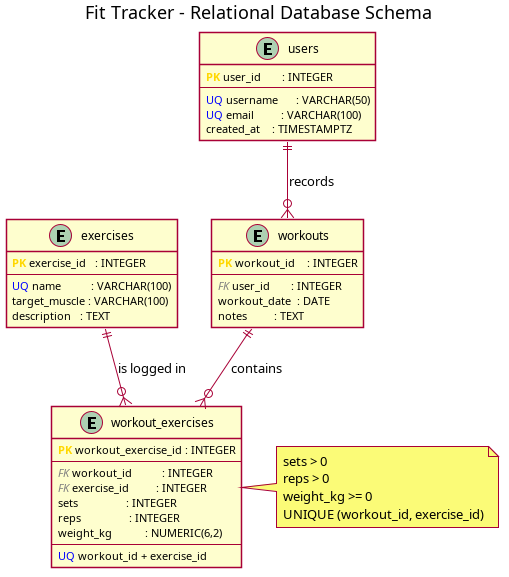
\includegraphics[width=0.88\linewidth]{01-database-schema.png}
  \caption{Relational schema implemented by \texttt{init.sql} and \texttt{models.py}.}
\end{figure}

\begin{center}
\small
\begin{tabularx}{\linewidth}{@{}>{\bfseries}p{0.21\linewidth} p{0.24\linewidth} X@{}}
\toprule
Table & Primary purpose & Important rules \\
\midrule
\texttt{users} & Owner of workouts & Unique username and email; generated identity. \\
\texttt{exercises} & Exercise dictionary & Unique name; muscle required; description optional. \\
\texttt{workouts} & One dated training session & Valid user required; deleting a referenced user is restricted. \\
\texttt{workout\_exercises} & Associative entity with performance data & Positive sets and reps, non-negative weight, unique exercise per workout. \\
\bottomrule
\end{tabularx}
\end{center}

The many-to-many relationship between workouts and exercises has attributes of
its own. It therefore becomes the associative entity
\texttt{workout\_exercises}, rather than an array or comma-separated column.
This keeps the design normalized and allows each performance to store sets,
repetitions and weight.

\subsection{Referential actions}

\begin{itemize}
  \item \texttt{users -> workouts}: \texttt{ON DELETE RESTRICT}. Existing history prevents accidental user deletion.
  \item \texttt{workouts -> workout\_exercises}: \texttt{ON DELETE CASCADE}. Deleting a workout also deletes its component entries.
  \item \texttt{exercises -> workout\_exercises}: \texttt{ON DELETE RESTRICT}. A dictionary entry used by history cannot be removed.
  \item Foreign-key updates cascade so an intentional identifier change remains consistent.
\end{itemize}

The same rules appear in both \filepath{init.sql} and \filepath{models.py}.
Whenever the database design changes, both representations and the tests must
be updated together.

\subsection{Domain and uniqueness constraints}

PostgreSQL rejects invalid data even if it bypasses the API:

\begin{lstlisting}[language=SQL,caption={Core database constraints}]
CHECK (sets > 0)
CHECK (reps > 0)
CHECK (weight_kg >= 0)
UNIQUE (workout_id, exercise_id)
\end{lstlisting}

The weight uses \texttt{NUMERIC(6,2)} rather than floating point. This preserves
two-decimal input without binary rounding errors. API validation adds upper
bounds of 100 sets, 1000 repetitions and 9999.99 kg.

\subsection{Initialization and persistent volumes}

PostgreSQL runs \filepath{init.sql} only when
\filepath{postgres\_data} is first created. The file creates all tables, inserts
user 1 and seeds 15 exercises. The final exercise insert uses:

\begin{lstlisting}[language=SQL]
ON CONFLICT (name) DO NOTHING;
\end{lstlisting}

This makes the seed statement safe to run manually, but editing
\filepath{init.sql} does not update an already initialized Docker volume. A
migration or explicit SQL command is required for existing installations.

\subsection{Workout volume query}

The history endpoint computes total training volume in the database:

\[
  \mathrm{volume} = \sum (\mathrm{sets} \times
  \mathrm{repetitions} \times \mathrm{weight\_kg}).
\]

The query uses an outer join and \texttt{COALESCE(..., 0)} so a newly created
workout without entries still appears with zero volume. Detail rows are then
joined to \texttt{exercises} to add the exercise name and target muscle.

\section{Backend implementation}

\subsection{Module responsibilities}

\begin{center}
\begin{tabularx}{\linewidth}{@{}>{\bfseries}p{0.22\linewidth} X@{}}
\toprule
Module & Responsibility \\
\midrule
\filepath{database.py} & Reads \texttt{DATABASE\_URL}, creates the engine and yields one SQLAlchemy session per request. \\
\filepath{models.py} & ORM classes, relationships, constraints and referential actions. \\
\filepath{schemas.py} & Request and response schemas, validation bounds and OpenAPI examples. \\
\filepath{main.py} & API-key dependency, four routes, queries, transactions and HTTP errors. \\
\bottomrule
\end{tabularx}
\end{center}

\subsection{HTTP contract}

\begin{center}
\small
\begin{tabularx}{\linewidth}{@{}p{0.11\linewidth} p{0.38\linewidth} p{0.10\linewidth} X@{}}
\toprule
Method & Path & Key & Success \\
\midrule
GET & \texttt{/exercises} & No & 200, sorted exercise array \\
GET & \texttt{/users/\{user\_id\}/workouts} & No & 200, joined history and volume \\
POST & \texttt{/workouts} & Yes & 201, created workout \\
POST & \texttt{/workouts/\{workout\_id\}/exercises} & Yes & 201, created performance entry \\
\bottomrule
\end{tabularx}
\end{center}

\begin{figure}[H]
  \centering
  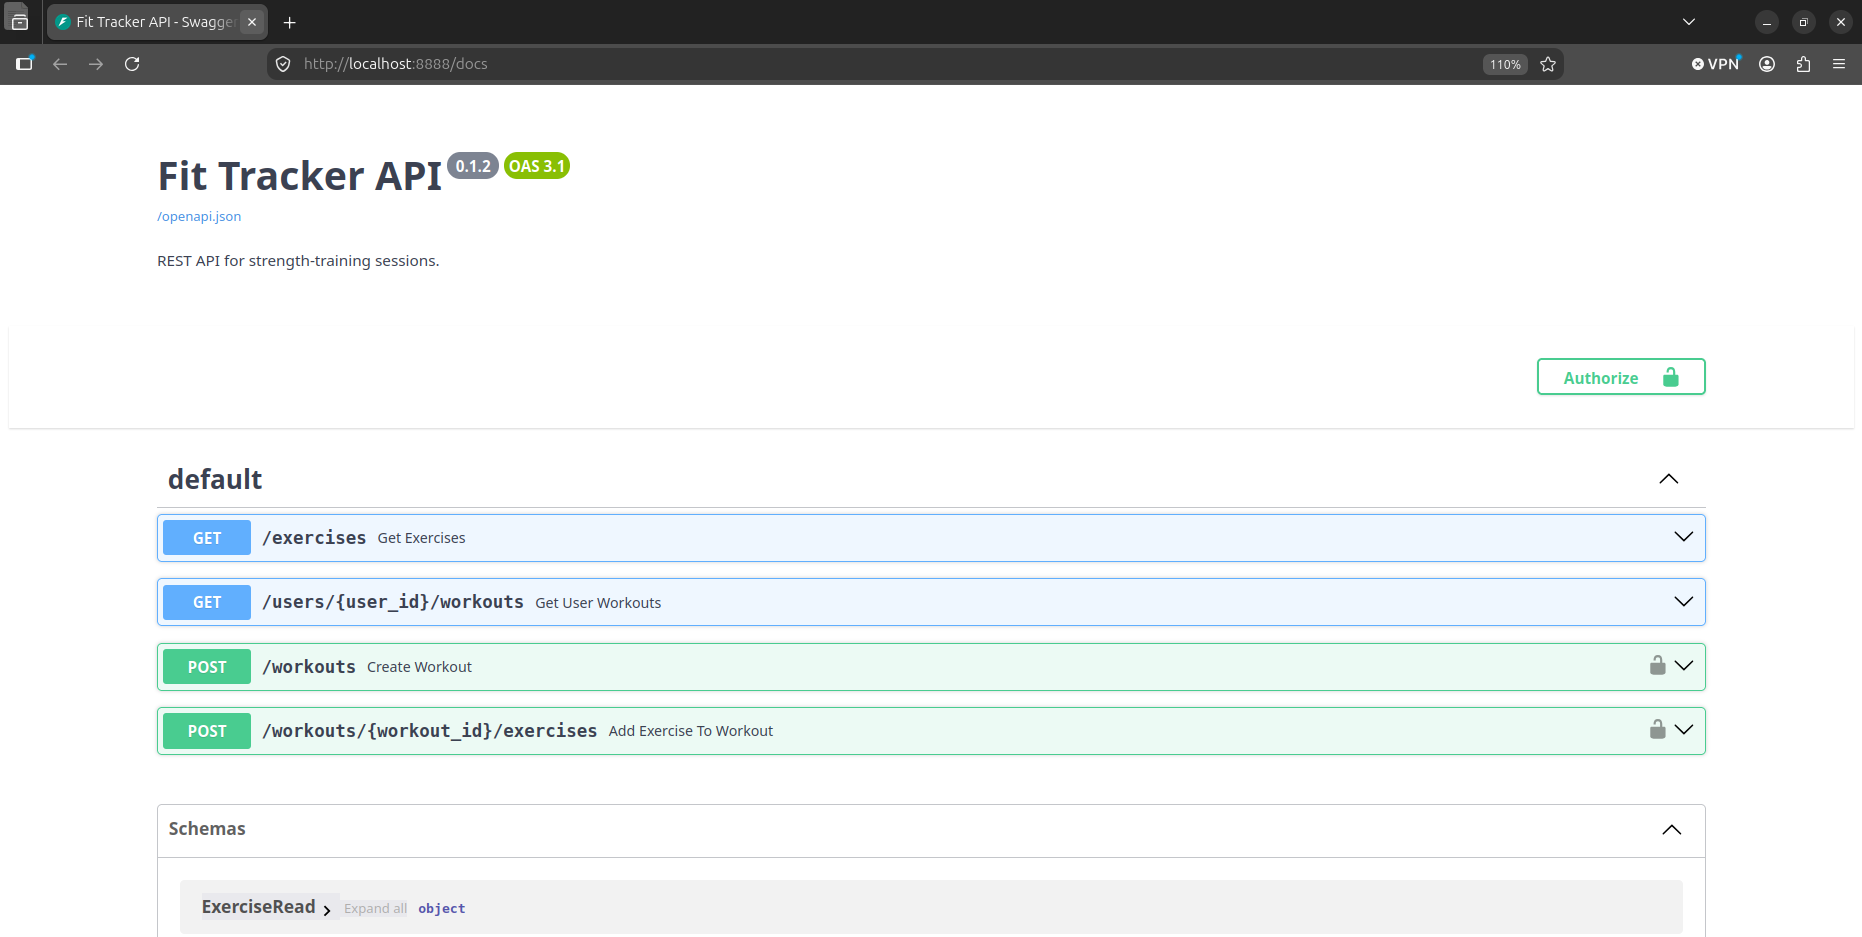
\includegraphics[width=0.94\linewidth]{02-swagger-api.png}
  \caption{FastAPI generates interactive OpenAPI documentation for the four routes.}
\end{figure}

\subsection{API-key authorization}

\filepath{main.py} reads the configured key when the module is imported.
Startup fails when the environment variable is missing. FastAPI's security
helper reads \texttt{X-API-Key}; \texttt{secrets.compare\_digest} performs the comparison. Protected routes use
the dependency declaratively, which also adds the authorization control to
Swagger UI.

\begin{infobox}
Public reads are a deliberate scope decision. Only the two POST routes require
the key. If reads later become private, apply the same dependency to them and
update both client and tests.
\end{infobox}

\subsection{Validation and error behavior}

Pydantic returns HTTP 422 before route code runs when a request violates a
schema. Route-level checks return meaningful errors:

\begin{itemize}
  \item 401 - missing or invalid API key;
  \item 404 - user, workout or exercise does not exist;
  \item 409 - the same exercise is logged twice in one workout; and
  \item 400 - a remaining database integrity error prevents the transaction.
\end{itemize}

All write handlers use \texttt{commit}, \texttt{rollback} after
\texttt{IntegrityError}, and \texttt{refresh} before returning the stored row.
Database sessions are always closed by the \texttt{get\_db} generator.

\subsection{Current transaction boundary}

Saving through the frontend performs one request to create the workout and
then one request per exercise. Those requests are separate transactions. If a
later exercise request fails, the workout and any earlier entries remain
stored. The UI reports this as a partial-workout error.

For an atomic future design, introduce a single request schema containing the
workout and all exercise entries, insert them in one database transaction, and
commit only after every entry succeeds. Keep the existing endpoints if
backward compatibility is required.

\section{Container deployment}

\subsection{Docker Compose services}

\begin{figure}[H]
  \centering
  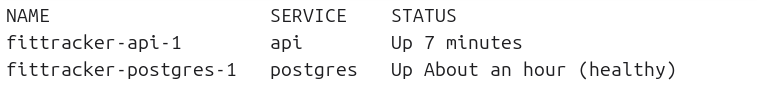
\includegraphics[width=0.82\linewidth]{03-docker-services.png}
  \caption{Expected PostgreSQL and API service state.}
\end{figure}

The \texttt{postgres} service uses PostgreSQL 15, a named volume and a
\texttt{pg\_isready} health check. The \texttt{api} service starts only after
that health check succeeds. Port 8000 inside the API container maps to
\texttt{API\_PORT}, normally 8888, on the host.

\subsection{Image hardening}

The API Dockerfile uses two stages. The builder creates a virtual environment
and installs dependencies. The runtime stage copies only the environment and
four application modules. It creates \texttt{appuser}, switches away from root
and starts Uvicorn on \texttt{0.0.0.0:8000}.

Verify the effective user with:

\begin{lstlisting}[caption={Checking the API container user}]
docker compose exec api whoami
# expected: appuser
\end{lstlisting}

\subsection{Configuration and secrets}

\filepath{.env.example} documents six required values. The real
\filepath{.env} is ignored by Git. The database password must be identical in
\texttt{POSTGRES\_PASSWORD} and in the password portion of
\texttt{DATABASE\_URL}. Never commit a real API key, password, database dump or
screenshot containing a secret.

\subsection{Operational commands}

\begin{lstlisting}[caption={Normal backend lifecycle}]
docker compose up -d --build
docker compose ps
docker compose logs -f api postgres
docker compose down
\end{lstlisting}

The final command preserves the named volume. \texttt{docker compose down -v}
deletes the project database and is therefore reserved for an intentional
reset or disposable CI environment.

\section{Desktop frontend}

\subsection{Module design}

\begin{center}
\small
\begin{tabularx}{\linewidth}{@{}>{\bfseries}p{0.30\linewidth} X@{}}
\toprule
File & Role \\
\midrule
\filepath{\_\_main\_\_.py} & Application controller, connect/disconnect lifecycle and Tk root. \\
\filepath{connection\_dialog.py} & URL and masked API-key input with syntax validation. \\
\filepath{api.py} & HTTP client, timeouts, JSON conversion and user-friendly errors. \\
\filepath{ui.py} & Three tabs, input validation, background tasks and result display. \\
\filepath{\_\_init\_\_.py} & Package metadata and version. \\
\bottomrule
\end{tabularx}
\end{center}

The UI receives an \texttt{ApiClient} instance instead of importing global
connection settings. This keeps HTTP behavior testable and avoids storing the
API key on disk.

\subsection{Threading and Tk safety}

Network calls must not block Tk's event loop. \filepath{ui.py} starts daemon
worker threads and places their results into a thread-safe queue. The Tk thread
polls the queue every 100 ms, updates widgets and displays message boxes. Worker
threads never manipulate Tk widgets directly.

\subsection{Client-side validation}

The desktop frontend checks the API URL, non-empty API key, positive user ID,
ISO date, sets, repetitions, weight range and duplicate pending exercises.
This improves feedback, while Pydantic and PostgreSQL remain the authoritative
validation layers.

\subsection{HTTP behavior}

\texttt{ApiClient} removes a trailing slash, requires HTTP or HTTPS, uses an
8-second timeout and sends the API key only for protected requests. It converts
FastAPI validation arrays into readable messages and distinguishes timeouts,
connection errors, HTTP errors and invalid JSON.

\section{Build and Debian packaging}

\subsection{Locked frontend environment}

\filepath{frontend/pyproject.toml} defines Python 3.11 or newer, \texttt{requests}
as the runtime dependency and PyInstaller plus pytest as development tools.
\filepath{frontend/uv.lock} records the resolved versions. Use:

\begin{lstlisting}
cd frontend
uv sync --frozen
uv run python -m fittracker_frontend
\end{lstlisting}

\subsection{Executable and package layout}

\texttt{make frontend-build} creates a windowed PyInstaller directory build.
\texttt{make deb} stages and packages it with \texttt{fpm}:

\begin{lstlisting}
/opt/fittracker/fittracker       executable and bundled libraries
/usr/bin/fittracker              symbolic link to the executable
/usr/share/applications/
  fittracker.desktop             desktop menu entry
\end{lstlisting}

The resulting file is
\filepath{frontend/dist/fittracker-frontend\_VERSION\_amd64.deb}. Validate it
with \texttt{make deb-info}, install it with \texttt{sudo apt install ./FILE},
and test the command from a directory outside the repository.

\subsection{Version synchronization}

Before a release, update the same semantic version in:

\begin{itemize}
  \item \filepath{Makefile} (\texttt{FRONTEND\_VERSION});
  \item \filepath{main.py} (FastAPI version);
  \item \filepath{frontend/pyproject.toml}; and
  \item \filepath{frontend/src/fittracker_frontend/\_\_init\_\_.py}.
\end{itemize}

Then run \texttt{uv lock} inside \filepath{frontend/} so the lock file contains
the same project version. A release tag must use the matching \texttt{vX.Y.Z}
form.

\section{Automated testing}

\begin{figure}[H]
  \centering
  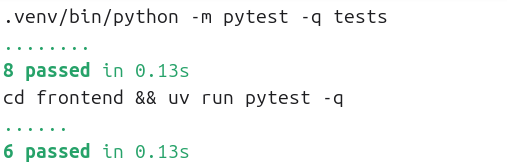
\includegraphics[width=0.76\linewidth]{04-automated-tests.png}
  \caption{Version 1.0.0 passes eight backend and six frontend tests.}
\end{figure}

Run both suites from the repository root:

\begin{lstlisting}
make test
\end{lstlisting}

\subsection{Backend tests}

The backend suite uses an in-memory SQLite database with foreign-key checks
enabled and overrides FastAPI's \texttt{get\_db} dependency. An automatic
fixture recreates the schema and seed rows for every test. The tests cover:

\begin{itemize}
  \item public exercise reads and joined history with correct volume;
  \item write authorization, request validation, 404 and 409 behavior; and
  \item database rejection of negative weight and orphan foreign keys.
\end{itemize}

SQLite keeps unit tests fast, while the CI Docker job verifies the real
PostgreSQL initialization and service connection.

\subsection{Frontend tests}

The frontend suite replaces \texttt{requests.request} with controlled response
objects. It checks URL validation, public GET headers, protected POST headers,
Decimal serialization, HTTP detail messages and connection failures without
requiring a display server.

\subsection{Adding a regression test}

Every bug fix should first receive the smallest failing test. Place API and
constraint tests in \filepath{tests/}; place HTTP-client behavior in
\filepath{frontend/tests/}. The test must fail before the fix, pass afterward,
and remain deterministic without external network access.

\section{Continuous integration and releases}

\subsection{CI workflow}

\begin{figure}[H]
  \centering
  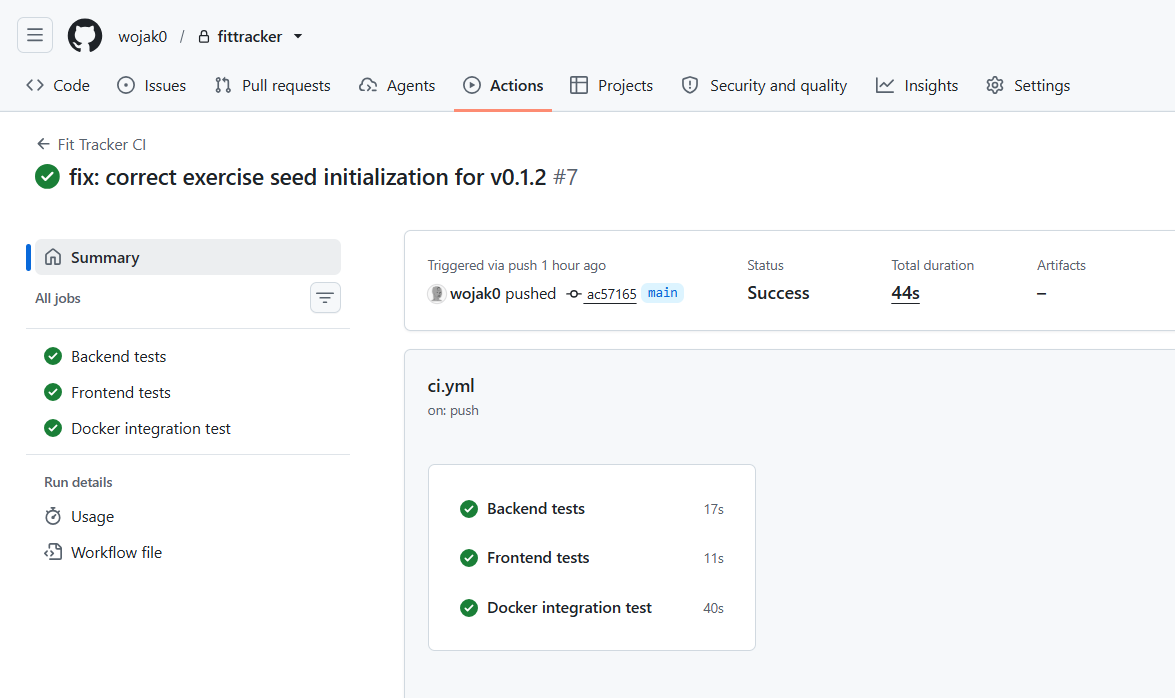
\includegraphics[width=0.92\linewidth]{05-github-actions.png}
  \caption{GitHub Actions verifies backend, frontend and Docker integration independently.}
\end{figure}

\filepath{.github/workflows/ci.yml} runs on pushes and pull requests to
\texttt{main}. Its three jobs are deliberately independent:

\begin{enumerate}
  \item backend tests install \filepath{requirements-dev.txt};
  \item frontend tests use the frozen uv environment; and
  \item Docker integration validates Compose, starts PostgreSQL and FastAPI,
        retries \texttt{/exercises}, prints logs on failure and removes the
        disposable CI volume.
\end{enumerate}

\subsection{Tagged Debian release}

\begin{figure}[H]
  \centering
  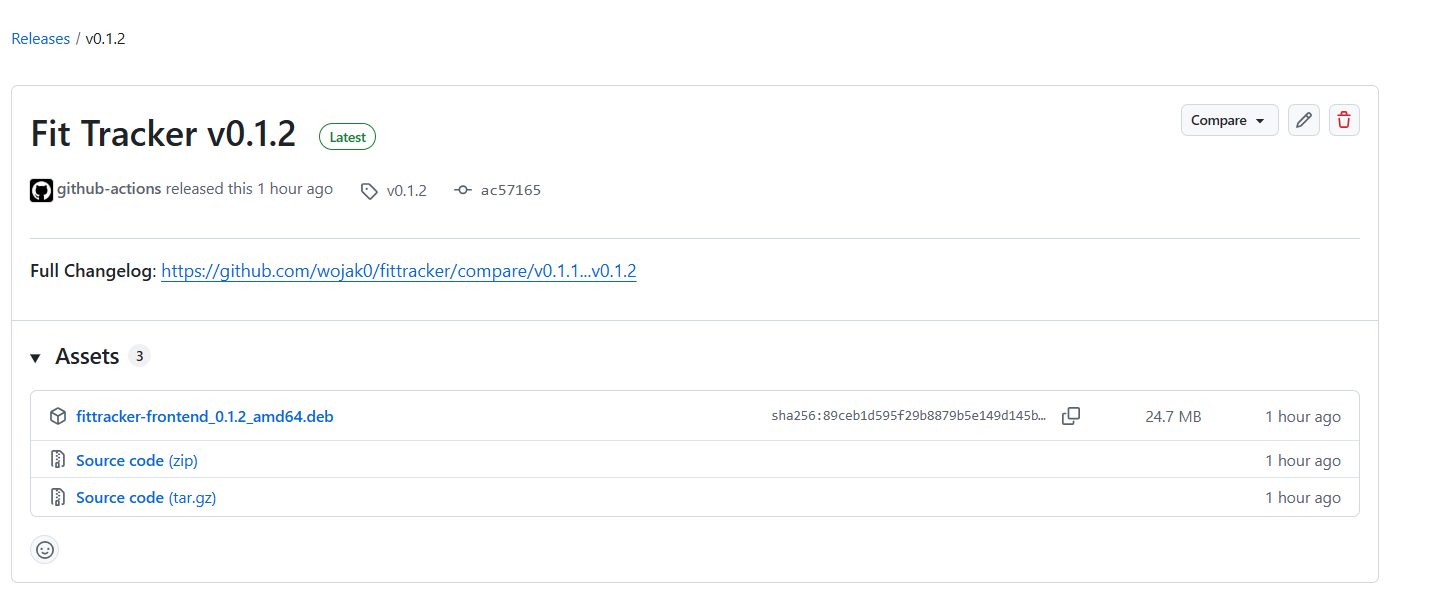
\includegraphics[width=0.92\linewidth]{06-github-release.png}
  \caption{A version tag publishes the validated amd64 Debian package as a release asset.}
\end{figure}

\filepath{.github/workflows/release.yml} may be started manually, but it
publishes a GitHub Release only for a tag matching \texttt{v*}. The job installs
build dependencies, runs \texttt{make deb}, inspects the package, uploads a CI
artifact and creates the release with generated notes.

\begin{lstlisting}[caption={Creating a normal release after green tests}]
git tag -a v1.0.0 -m "Fit Tracker v1.0.0"
git push origin v1.0.0
\end{lstlisting}

Never move an existing release tag. Correct the source, increment the version
and create a new tag.

\section{Developer workflows}

\subsection{Initial local setup}

\begin{lstlisting}
cp .env.example .env
nano .env
docker compose up -d --build
python3 -m venv .venv
.venv/bin/python -m pip install -r requirements-dev.txt
cd frontend && uv sync --frozen && cd ..
make test
\end{lstlisting}

Use unique local secrets. The API container reads changes to environment
variables only when it is recreated.

\subsection{Change checklist}

For each implementation change:

\begin{enumerate}
  \item update the smallest relevant source modules;
  \item keep SQL, ORM models and schemas consistent;
  \item add or update automated tests;
  \item run \texttt{git diff --check} and \texttt{make test};
  \item run a clean Docker integration check when database or backend code changes;
  \item update the manuals and version if user-visible behavior changes; and
  \item commit a focused change and confirm GitHub Actions is green.
\end{enumerate}

\section{Data administration}

\subsection{Add an exercise}

Add the row to the seed list in \filepath{init.sql} for new installations. To
update an existing volume without deleting history, execute an idempotent
insert:

\begin{lstlisting}[language=SQL]
INSERT INTO exercises (name, target_muscle, description)
VALUES ('Pull-Up', 'Back', 'Bodyweight vertical pulling exercise.')
ON CONFLICT (name) DO NOTHING;
\end{lstlisting}

Run SQL safely through the container:

\begin{lstlisting}
docker compose exec postgres sh -c \
  'psql -U "$POSTGRES_USER" -d "$POSTGRES_DB"'
\end{lstlisting}

The quoted command expands the database variables inside the PostgreSQL
container instead of requiring them to be exported by the host shell. Refresh
the frontend dictionary after insertion.

\subsection{Add another user}

Version 1.0.0 has no registration route. An administrator can insert a user:

\begin{lstlisting}[language=SQL]
INSERT INTO users (username, email)
VALUES ('second_user', 'second@example.invalid')
RETURNING user_id;
\end{lstlisting}

The returned identifier can be entered in the frontend's User ID field. A
production multi-user design should add authenticated registration and must
not rely on manually selecting arbitrary user IDs.

\subsection{Backup and restore}

Create a logical SQL backup without stopping the services:

\begin{lstlisting}
docker compose exec -T postgres sh -c \
  'pg_dump -U "$POSTGRES_USER" "$POSTGRES_DB"' \
  > fittracker-backup.sql
\end{lstlisting}

Treat the dump as sensitive because it contains user and workout data. Test
restoration in a separate disposable Compose project before depending on a
backup. Do not commit dumps to Git.

\subsection{Intentional reset}

\begin{warnbox}
\texttt{docker compose down -v} permanently deletes the current named volume.
Create and verify a backup first. A normal shutdown uses
\texttt{docker compose down} without \texttt{-v}.
\end{warnbox}

\section{Planned extension points}

\subsection{Delete a workout}

The database already cascades deletion from a workout to its performance
entries. A safe feature requires all of the following:

\begin{enumerate}
  \item add \texttt{DELETE /workouts/\{workout\_id\}} protected by the API key;
  \item return 404 for an unknown workout and 204 after deletion;
  \item ensure the requested workout belongs to the intended user;
  \item add backend authorization, cascade and not-found tests;
  \item add a selected-history delete button with an explicit confirmation; and
  \item refresh the history only after a successful response.
\end{enumerate}

Do not implement deletion only in the GUI or by connecting the client directly
to PostgreSQL.

\subsection{User registration and authentication}

Add request schemas, unique-conflict handling and endpoints for users. For a
networked or public deployment, replace the shared write key with per-user
authentication, password hashing or an external identity provider, and enforce
ownership on every workout query and mutation.

\subsection{New measurements or goals table}

A future \texttt{body\_measurements} table can reference \texttt{users} and
store a measurement date, body weight and optional note. Introduce it with a
real migration tool such as Alembic; do not edit a live database manually and
assume \filepath{init.sql} performed the migration.

\subsection{Android client}

An Android application can reuse the HTTP API; the PostgreSQL and FastAPI
backend still must run on a reachable computer or server. The phone must use
that host's LAN or HTTPS address instead of \texttt{localhost}, and firewall,
TLS and secret storage must be addressed. An Android installer would be an APK,
not the Debian package.

\section{Security and reliability notes}

\begin{itemize}
  \item Keep \filepath{.env}, backups and real credentials outside Git.
  \item Use HTTPS and a reverse proxy before exposing the API beyond a trusted network.
  \item Replace development keys before demonstrations or deployments.
  \item Keep the API container non-root and dependencies within supported ranges.
  \item Validate at three levels: frontend feedback, Pydantic contract and database constraints.
  \item Review logs without copying secrets into issues, screenshots or manuals.
  \item Back up persistent data before schema changes or destructive commands.
\end{itemize}

\section{Known limitations}

Version 1.0.0 intentionally does not provide workout editing or deletion, user
registration, per-user login, database migrations, a web frontend, an Android
client or HTTPS termination. The current API creates a workout before its
exercise entries and therefore cannot guarantee whole-session atomicity across
multiple requests. These limitations do not prevent the approved DBMS workflow,
but they define the boundary for future development.

\newpage
\section{Handover checklist}

Before handing a new version to another developer, confirm:

\begin{enumerate}
  \item the repository is clean and contains no \filepath{.env} or generated secrets;
  \item schema SQL, ORM models, API schemas and diagram agree;
  \item \texttt{make test} passes all backend and frontend tests;
  \item a fresh Docker volume initializes, becomes healthy and exposes 15 exercises;
  \item the API container runs as \texttt{appuser};
  \item the Debian package builds, installs and starts outside the source tree;
  \item user-visible behavior matches the User Manual;
  \item GitHub CI and the tagged release workflow are green; and
  \item version numbers and release filenames match.
\end{enumerate}

\subsection*{Maintenance impact map}

\begin{center}
\small
\begin{tabularx}{\linewidth}{@{}>{\bfseries}p{0.24\linewidth} X@{}}
\toprule
Change & Sources and verification that normally change with it \\
\midrule
Database structure & \filepath{init.sql}, \filepath{models.py}, \filepath{schema.puml}, constraint tests and clean-volume initialization. \\
API contract & \filepath{schemas.py}, \filepath{main.py}, frontend API client, backend tests and both manuals. \\
Frontend behavior & UI module, frontend tests, User Manual instructions and screenshots. \\
Release version & Makefile, FastAPI metadata, frontend package metadata, uv lock file, tag and release filename. \\
Dependencies & Requirements or pyproject, lock file where applicable, local tests and container or package rebuild. \\
Deployment behavior & Dockerfile, Compose file, Make targets, CI integration job and clean-machine procedure. \\
\bottomrule
\end{tabularx}
\end{center}

\begin{beispielbox}
The implementation remains maintainable when every change preserves the same
chain of responsibility: the GUI collects intent, the API validates and
authorizes it, SQLAlchemy manages the transaction, and PostgreSQL protects the
data model.
\end{beispielbox}

\end{document}
